\documentclass[11pt]{article}

% Pacotes
\RequirePackage{luatex85}
\usepackage{amsmath}
\usepackage{amssymb}
\usepackage{graphicx}
\usepackage[colorlinks=true, allcolors=blue]{hyperref}
\usepackage{amsthm}
\usepackage{framed, color,xcolor}
\usepackage{stmaryrd}
\usepackage{rotating}           % Usado para rotacionar o texto
\usepackage[all,knot,arc,import,poly]{xy}   % Pacote para desenhos gráficos
% Este pacote pode conflitar com outros pacotes gráficos como o ``pictex''
% Então é necessário usar apenas um dos pacotes conflitantes
\usepackage{tikz, tikz-cd}
\usepackage{epigraph}
\usetikzlibrary{babel}
\usetikzlibrary{positioning}
\usetikzlibrary{calc}
\usepackage[stix2]{newtxmath}
\usepackage{mathtools, nccmath}
%\usepackage[usenames,dvipsnames]{xcolor}
\usepackage{amssymb, mathrsfs}
\usepackage[numbers]{natbib}
\usepackage{fontspec}
\usepackage{enumitem} % pra substituir o símbolo do itemize por alguma coisa legal, tipo setinhas:  \begin{itemize}[label=\ding{212}]
\usepackage{pifont}
\usepackage{stmaryrd} % for \arrownot (notação de adjacência em grafo)
\usepackage{quiver} %pacote do quiver pra desenhar diagramas mais legais

%Fontes e Línguas
\usepackage[portuguese]{babel}
%\usepackage{eufrak}
\usepackage{emoji}
\setmainfont{DarwinSerif-Regular.otf}
\newfontfamily\fakebold[FakeBold=1.75]{DarwinSerif-Regular.otf}
\newfontfamily\fakeitalic[FakeSlant=0.2]{DarwinSerif-Regular.otf}
\renewcommand{\textbf}[1]{{\fakebold#1}}
\renewcommand{\textit}[1]{{\fakeitalic#1}}
\renewcommand{\bfseries}{\fakebold}
\renewcommand{\itshape}{\fakeitalic}



%Cores


%Comandinhos que gosto
\usepackage{mathtools}
\newcommand{\defeq}{\vcentcolon=}
\newcommand{\eqdef}{=\vcentcolon}
\newcommand{\bigslant}[2]{{\raisebox{.2em}{$#1$}\left/\raisebox{-.2em}{$#2$}\right.}}
\newcommand{\logo}{\Rightarrow}
\newcommand{\pulinho}{\vspace{.5cm}}
\newcommand{\edge}{%
  \mathrel{-}% minus as a relation
  \joinrel\joinrel % some backup
  \mathrel{-}% minus as a relation
}
\newcommand{\notedge}{%
  \mathrel{\mkern2mu}% a small advancement
  \arrownot % a short slash
  \mathrel{\mkern-2mu}% compensate
  \edge
}

\newcommand{\Aut}{\text{Aut}}
\newcommand{\Cay}{\text{Cay}}

\newcommand{\luafacil}{
\emoji{waxing-crescent-moon}
}

\newcommand{\luamedio}{
\emoji{first-quarter-moon}
}

\newcommand{\luadificil}{
\emoji{waxing-gibbous-moon}
}

\newcommand{\luaprojeto}{
\emoji{full-moon}
}

\let\varphi\phi

%Caixinhas coloridas

\theoremstyle{definition}
\newtheorem{theorem}{Teorema}
\newenvironment{teorema}{
\definecolor{shadecolor}{HTML}{f59aa3}
\begin{shaded}
\begin{theorem}
}
{
\end{theorem}
\end{shaded}
}

\theoremstyle{definition}
\newtheorem*{theorem*}{Teorema}
\newenvironment{teorema*}{
\definecolor{shadecolor}{HTML}{f59aa3}
\begin{shaded}
\begin{theorem*}
}
{
\end{theorem*}
\end{shaded}
}

\theoremstyle{definition}
\newtheorem{prop}{Proposição}
\newenvironment{proposicao}{
\definecolor{shadecolor}{HTML}{FFDBDF}
\begin{shaded}
\begin{prop}
}
{
\end{prop}
\end{shaded}
}

\theoremstyle{definition}
\newtheorem*{prop*}{Proposição}
\newenvironment{proposicao*}{
\definecolor{shadecolor}{HTML}{FFDBDF}
\begin{shaded}
\begin{prop*}
}
{
\end{prop*}
\end{shaded}
}

\theoremstyle{definition}
\newtheorem{cor}{Corolário}
\newenvironment{corolario}{
\definecolor{shadecolor}{HTML}{f59aa3}
\begin{shaded}
\begin{cor}
}
{
\end{cor}
\end{shaded}
}

\theoremstyle{definition}
\newtheorem*{cor*}{Corolário}
\newenvironment{corolario*}{
\definecolor{shadecolor}{HTML}{f59aa3}
\begin{shaded}
\begin{cor*}
}
{
\end{cor*}
\end{shaded}
}



\theoremstyle{definition}
\newtheorem{definition}{Definição}
\newenvironment{definicao}{
\definecolor{shadecolor}{HTML}{defcfc}
\begin{shaded}
\begin{definition}
}
{
\end{definition}
\end{shaded}
}

\theoremstyle{definition}
\newtheorem*{definition*}{Definição}
\newenvironment{definicao*}{
\definecolor{shadecolor}{HTML}{defcfc}
\begin{shaded}
\begin{definition*}
}
{
\end{definition*}
\end{shaded}
}

\theoremstyle{definition}
\newtheorem{example}{Exemplo}
\newenvironment{exemplo}{
\definecolor{shadecolor}{HTML}{b9e6d3}
\begin{shaded}
\begin{example}
}
{
\end{example}
\end{shaded}
}

\theoremstyle{definition}
\newtheorem*{example*}{Exemplo}
\newenvironment{exemplo*}{
\definecolor{shadecolor}{HTML}{b9e6d3}
\begin{shaded}
\begin{example*}
}
{
\end{example*}
\end{shaded}
}

\theoremstyle{definition}
\newtheorem{veronica}{Lema}
\newenvironment{lema}{
\definecolor{shadecolor}{HTML}{FFF1F2}
\begin{shaded}
\begin{veronica}
}
{
\end{veronica}
\end{shaded}
}

\theoremstyle{definition}
\newtheorem*{veronica*}{Lema}
\newenvironment{lema*}{
\definecolor{shadecolor}{HTML}{FFF1F2}
\begin{shaded}
\begin{veronica*}
}
{
\end{veronica*}
\end{shaded}
}

\newenvironment{prova}{\paragraph{Demonstração:}}{\hfill$\square$ 
\pulinho
}

\newenvironment{aviso}{
\definecolor{shadecolor}{HTML}{fffe9a}
\begin{shaded}
}{\end{shaded}}

\theoremstyle{definition}
\newtheorem{exersisio}{Exercício}
\newenvironment{exercicio}{
\definecolor{shadecolor}{HTML}{CFB5FF}
\begin{shaded}
\begin{exersisio}
}
{
\end{exersisio}
\end{shaded}
}

%Tamanho do papel
\usepackage[a4paper,top=1cm,bottom=1cm,margin=3.5cm]{geometry}



%%%%%%%%%%%%%%%%%%%%%%%%%%%%%%%%%%%%%%%%%%%%%%%


%Definições só pra esse texto
\usepackage[bb=boondox]{mathalpha}

\title{Capítulo 1 - Grafos infinitos na natureza}
\author{Violeta Mar}
\date{}

\begin{document}
\maketitle
\begin{center}
        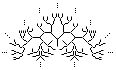
\includegraphics[scale=2.5]{desenhos/binariainfinita.png}
\end{center}
Grafos no nosso dia-a-dia tendem a ser finitos. Geralmente os conhecemos com o nome mais popular de redes: redes de interações ecológicas, redes de modens conectando computadores e celulares pelo mundo, redes sociais, redes de sinapses entre neurônios. São objetos discretos conectados abstratamente por algum tipo de relação, e visualmente são pontinhos ligadas por linhas. Nesse mundo globalizado profundamente interconectado, todo mundo anda estudando redes e tentando extrair informações delas. Nesse livro, não estamos interessados em nada disso. Com a liberdade do pensamento abstrato, permitimos nos fantasiar com redes que tenham infinitos nódulos e infinitas conexões. Mas existe isso mesmo?

Depende do que você considera como existir. Firmemente postulamos de começo a fé na dimensão platônica da realidade, onde do lado de amoreiras, micro-organismos, rochas metamórficas e pessoas existem também ordinais transfinitos, modelos contáveis de ZFC, simetrias de tesselações do plano hiperbólico e grafos infinitos. Nessa visão estendida de natureza, em que biomas vamos nos tropeçar com grafos infinitos? Vários, mas nesse livro vamos restringir nossas andanças para os mundos da lógica e da álgebra, áreas que a autora (eu) particularmente gosta. Nesse primeiro capítulo, introduziremos conceitos básicos ao lado de dois exemplos de grafos infinitos: o Grafo Contável (comumente conhecido como grafo de Rado ou o Grafo Aleatório), e grafos de simetrias (comumente conhecidos como grafos de Cayley).

De uma vez por todas, como todo bom matemático, definimos nosso objeto principal.

\begin{definicao*}[Grafos]
Um grafo $G$ consiste de um par de conjuntos $V,A$, onde $A$ é um subconjunto de $V\times V$ tal que $(v,w) \in A$ implica em $(w,v) \in A$ e $(v,v) \notin A$ pra todos $v,w \in V$. Os elementos de $V$ são chamados vértices e os de $A$ arestas. Quando existe uma aresta entre dois vértices $v$ e $w$, dizemos que eles são adjacentes e denotamos como $v \edge w$.
    \begin{center}
        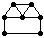
\includegraphics[scale=2]{desenhos/casinha.png}
\end{center}

\end{definicao*}

Veja que nesta definição não existem arestas que ligam um vértice a ele mesmo, nem mais que uma aresta entre dois vértices. Poderíamos ter dado uma definição alternativa que permitiriam essas coisas, que seriam então objetos geralmente chamados de multigrafos. Uma outra variante de grafo que iremos falar vão ser os grafos direcionados, que são grafos onde cada aresta possui um direcionamento apontando para um dos lados. Para obter os grafos direcionados, basta tirar a primeira condição da nossa definição anterior, a de simetria. Daí, $(v,w) \in A$ dirá então que temos uma seta de $v$ para $w$.

\section{O grafo de todos os grafos}

Nosso primeiro exemplo de grafo infinito vai ser um grafo que contém todos os possíveis exemplos do menor infinito possível: um grafo universal, que contém dentro dele, de forma não trivial, todos os outros grafos contáveis. Por isso, o chamamos com o artigo definitivo de o Grafo Contável. Pra chegar lá, como toda a vida, começamos com raízes. Quando desenhamos um grafo sem ciclos, ele naturalmente se parece com padrões de ramificações naturais, como sistemas de raízes, rizomas ou árvores. Tradicionalmente, o nome árvore se fixou, e é este que usamos. Primeiro, vamos clarificar o que queremos dizer com ciclos (é o que você está pensando mesmo).

\begin{definicao*}[Caminhos, ciclos e conexidade]
    Um caminho em um grafo é uma sequência de vértices distintos $v_1, \dots, v_n$ onde cada $v_i$ é adjacente ao $v_{i+1}$.

    \begin{center}
        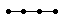
\includegraphics[scale=2]{desenhos/caminho.png}
\end{center}
    
    Um ciclo é um caminho onde $v_1 = v_n$. 

    \begin{center}
        
\includegraphics[scale=2]{desenhos/ciclo.png}
\end{center}
    
    Um grafo é conexo quando existe pelo menos um caminho entre todos os seus vértices.
\end{definicao*}

Para facilitar nossa vida, vamos geralmente estar pensando em grafos conexos (grafos não conexos são só vários grafos conexos um do lado do outro, e aí nossos teoremas teriam que ficar lidando com estas componentes conexas, o que tende a ser fácil de ver mas chato de escrever).

\begin{definicao*}[Árvores e raízes]
    Um grafo conexo sem ciclos é chamado de árvore. Uma árvore enraizada é um par composto de uma árvore e um vértice desta árvore, que chamamos de raiz.

    \begin{center}
        
\includegraphics[scale=2]{desenhos/arvre.png}
\end{center}
\end{definicao*}

Enraizar uma árvore é dar um começo pra ela. Isto é útil de diversas maneiras.

\begin{exercicio}
    \luafacil Mostre que a condição de ser árvore é equivalente a existência de um e apenas um caminho entre quaisquer dois vértices.
\end{exercicio}

Veja que esse exercício mostra que dado uma árvore enraizada, cada vértice pode ser identificado com seu único caminho chegando a raiz.

Vamos introduzir mais uma noção que vai continuar a aparecer pelo resto do livro: simetria. É um conceito elusivo na linguagem comum, mas na matemática usamos com uma definição bem precisa. Uma simetria de um objeto matemático é algum tipo de transformação que podemos aplicar nele que, ao final, deixa o objeto com a mesma cara que ele tinha antes (procure uma flor com quatro pétalas e veja que se a rodarmos noventa graus, ela parece a mesma).

\begin{center}
        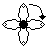
\includegraphics[scale=2]{desenhos/fro.png}
\end{center}

Na perspectiva conjuntista usual da matemática, formalizamos essa noção de transformação como uma bijeção do objeto nele mesmo que mantém a estrutura dele invariante. No caso de grafos, vamos ter uma bijeção do grafo nele mesmo que preserva a sua estrutura, ou seja, leva vértices em vértices e arestas em arestas de forma que vértices conectados entre si são levados em vértices conectados entre si. Uma forma equivalente de se ver é que estamos trocando os nomes dados a nossos vértices sem perder nenhuma informação. Por exemplo, no grafo a seguir, podemos trocar os nomes dos vértices $C$ e $D$, e qualquer afirmação referente a estrutura do grafo que era verdade antes da troca de nomes continua verdade após a troca de nomes. Geometricamente, podemos visualizar esta simetria como uma reflexão.

\begin{center}
        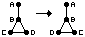
\includegraphics[scale=2]{desenhos/refrexao.png}
\end{center}

Juntamos todas estas bijeções em um único conjunto, o conjunto dos chamados automorfismos do grafo. O truque de mágica é perceber que podemos juntar estes automorfismos entre si pra obter novos automorfismos. Basta aplicar duas transformações uma atrás da outra: compor. Da mesma forma que codificamos a estrutura da aritmética abstraindo números como conjuntos abstratos de entidades com operações de soma e produto comportadas da forma que esperamos (com os axiomas de Peano, ou então com os axiomas de anéis e corpos da álgebra abstrata), codificamos a estrutura da simetria abstraindo o conceito de transformações que deixam objetos invariantes como um conjunto abstrato com uma operação de composição bem comportada - este é o conceito de um grupo. Surpreendentemente, três axiomas já são suficientes.

\begin{definicao*}[Grupo]
    Um grupo $G$ é um conjunto munido de uma operação associativa ($(ab)c = a(bc)$), com identidade (existe $e$ tal que $ea = ae = a$ pra todo $a \in G$) e com inversos (pra todo $a \in G$ existe $b \in G$ tal que $ab = e$).
\end{definicao*}

Infelizmente, grafos e grupos, nossos dois objetos de estudo, começam com a mesma letra, então às vezes $G$ é grafo e às vezes $G$ é grupo. Se acostume com a confusão.


\begin{definicao*}[Grupo de automorfismos]
    Um automorfismo $\varphi: G \rightarrow G$ de um grafo $G$ é uma bijeção de seu conjunto de vértices de forma que $v \edge w$ se e somente se $\varphi(v) \edge \varphi(w)$. O conjunto $\Aut (G)$ munido da operação de composição de funções é um grupo, chamado de grupo de automorfismos de $G$.
\end{definicao*}

Nessa definição, não fizemos menção a bijeção entre as arestas que deveria também existir. É claro, se temos uma bijeção entre vértices que respeita a relação de adjacência, temos também uma bijeção entre as arestas que preserva adjacência de arestas (isto é, ela leva arestas que compartilham um vértice em arestas que compartilham um vértice).

\begin{exercicio}
    \luafacil Mostre isso.
\end{exercicio}

Você poderia se perguntar porque não fizemos o contrário, isto é, começamos com uma bijeção de arestas e obtemos uma bijeção de vértices. Surpreendentemente (pra mim, pelo menos), alguns grafos admitem uma bijeção de arestas que não induz uma bijeção de vértices.

\begin{exercicio}
    \luamedio Encontre pelo menos um grafo que possui uma bijeção entre arestas que preserva adjacência mas que não induz uma bijeção entre vértices que preserva adjacência. (Dica: ele terá que ter 4 vértices)
\end{exercicio}

A transformação que não faz nada, isto é, a identidade $id(v) = v$ é a simetria trivial, presente em qualquer $\Aut(G)$ (ela é o objeto identidade necessário pra definição de grupo). Estruturas matemáticas que não possuem nenhuma simetria fora a trivial geralmente são chamados de rígidos. 

Vamos voltar agora para as árvores enraizadas. Como elas possuem um ponto distinguido, sua raiz, é natural considerarmos as simetrias que fixam a raiz. Pra construir o Grafo Contável, vamos querer olhar pra árvores enraizadas bem assimétricas - as rígidas.

\begin{definicao*}[Árvores enraizadas rígidas]
    Seja $T$ uma árvore enraizada e $r$ sua raiz. Dizemos que $\varphi \in \Aut(T)$ é um automorfismo de árvore enraizada se $\varphi(r) = r$. Chamamos $T$ de rígida se o único automorfismo de árvore enraizada é a identidade.
\end{definicao*}

\begin{exemplo*}
Esta é uma árvore rígida - a raiz é o vértice mais embaixo, como convencionaremos em todos os nossos desenhos.

    \begin{center}
        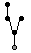
\includegraphics[scale=2]{desenhos/arvorerigida.png}
\end{center}
 
Se adicinarmos um vértice adjacente ao vértice mais à direita, criamos uma simetria (reflexão no eixo central da raiz), e assim ela não é mais rígida.

\begin{center}
        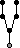
\includegraphics[scale=2]{desenhos/arvorenaorigida.png}
\end{center}
\end{exemplo*}

Tome uma árvore enraizada rígida $T$.

\begin{center}
        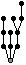
\includegraphics[scale=2]{desenhos/arvorerigidamae.png}
\end{center}

Apague a raiz, e as arestas que ligavam essa raiz a seus vizinhos. Vai restar alguns grafos não conectados entre si. 

\begin{center}
        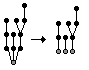
\includegraphics[scale=2]{desenhos/filhas.png}
\end{center}

Todos serão árvores também, e as enraizamos considerando o vértice que era vizinho da raiz original como sua nova raiz. Chame estas novas árvores de filhas de $T$.

\begin{exercicio}
    \luafacil Se convença que as filhas de $T$ também são rígidas.
\end{exercicio}

Vamos finalmente construir o Grafo Contável. Seu conjunto de vértices é o conjunto de todas as árvores enraizadas rígidas finitas. Dois vértices com árvores respectivas $T_1$ e $T_2$ serão ligados por uma aresta se ou $T_1$ é filha de $T_2$ ou $T_2$ é filha de $T_1$ (importante: não estamos colando estas árvores entre si pra formar o Grafo Contável. Estamos apenas usando as árvores para nomear vértices e decidirmos quando um está ligando o outro).

Construção esquisita. Vamos dar uma guinada pra outra direção e construir este mesmo grafo de outro jeito.

Imagine que você tenha muitas caixas vazias, de todos os tamanhos possíveis, e você quer brincar de encaixar caixas em outras caixas (porque não?). A primeira possibilidade é ter simplesmente uma caixa vazia. Você consegue colocar esta caixa vazia em uma outra caixa maior. Agora, você pode colocar esta caixa que contém uma caixa vazia em outra caixa. Mas também pode colocar a caixa que contém uma caixa vazia em uma caixa junto com outra caixa vazia em uma caixa... 

\begin{center}
        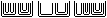
\includegraphics[scale=2.5]{desenhos/boxeswithinboxes.png}
\end{center}

Caixas não são a melhor analogia pra o que queremos fazer, na verdade... O que queremos são conjuntos, na interpretação matemática usual. No dia zero, $V_0$, temos apenas o conjunto vazio $\varnothing$. No primeiro dia, $V_1$, temos o conjunto vazio (que vem do dia anterior) e o conjunto que contém o vazio $\{\varnothing\}$. No segundo dia $V_2$, temos os dois conjuntos dos dias anteriores e mais $\{\varnothing, \{\varnothing\}\}$ e $\{\{ \varnothing\}\}$. No terceiro dia $V_3$, temos os quatro conjuntos dos dias anteriores mais $12$ novos para completarmos as $16$ possibilidades. Temos aqui um processo indutivo onde o dia seguinte $V_{i+1}$ é o conjunto de partes $\mathcal{P}(V_i)$, ou seja, todos os possíveis conjuntos formados com conjuntos do dia anterior. Chamamos de $V_\omega$ a união de todos os $V_i$, e seus elementos são ditos os conjuntos hereditariamente finitos (se já sabe sobre ordinais, veja que nada impeça que façamos este processo transfinitamente - assim construímos a chamada hierarquia de Von Neumann).

Agora, defina um grafo cujo conjunto de vértices é $V_\omega$ e dois vértices $X,Y$ estão ligados por uma aresta se $X \in Y$ ou se $Y \in X$.

Consegue ver que este grafo é o mesmo que o anterior?

\begin{proposicao}[Equivalência entre conjuntos hereditariamente finitos e árvores enraizadas rígidas finitas]
    Existe uma bijeção $f$ entre conjuntos hereditariamente finitos e árvores enraizadas rígidas finitas. Esta bijeção leva a relação de pertencimento na relação de filha, isto é, $X \in Y$ se e somente se $f(X)$ é filha de $f(Y)$.
\end{proposicao}
\begin{prova}
    Construímos a bijeção por indução. Primeiramente, associe ao conjunto vazio a árvore composta por um único vértice. Agora, suponha que já temos uma associação injetiva de $V_i$ (os conjuntos nascidos até o dia $i$) nas árvores enraizadas rígidas finitas. Tome um conjunto $X$ nascido no dia $i + 1$. $X$ deve ser um conjunto de finitos elementos, todos nascidos em dias anteriores, isto é, em $V_i$. Seja então $X = \{x_1, \dots, x_n\}$. Cada um destes $x_j$ possui uma árvore associada $T_i \defeq f(x_i)$. Coloque todas estas árvores uma do lado da outra, e ligue todas as suas raízes a um único novo vértice $r$. Chame esse novo grafo de $T$ e tome $r$ como a raiz. Este grafo é uma árvore finita, e não é muito difícil ver que ela deve ser rígida. 
    
    De fato, um automorfismo $\phi$ que fixa a raiz deve mandar vizinhos da raiz em vizinhos da raiz, e logo deve mandar uma das árvores $T_i$ em outra $T_{i'}$, definindo um isomorfismo entre elas. Mas supomos que a associação era injetiva, logo $i = i'$. Assim $\phi$ restrita a $T_i$ define um automorfismo que fixa raiz de $T_i$, que é rígida, logo $\phi$ é a identidade em todas as subárvores $T_i$ e portanto $\phi = id$ em toda a árvore $T$.

    $f$ vai ser sobrejetiva: suponha por indução que todas as árvores enraizadas rígidas finitas com número de vértices $\leq n$ estão na imagem. Dado uma árvore $T$ com $n +1$ vértices, suas filhas $T_1, \dots, T_k$ terão $\leq n$ vértices e portanto estarão associadas a conjuntos $X_1,\dots, X_k$. Junte estes em um conjunto $X = \{X_1, \dots, X_k\}$ e assim $f(X) = T$.

    A forma como construímos $f$ deixa claro que a relação de pertencimento é levada na relação de filha.
    
\end{prova}

Se a demonstração não te convenceu, faça alguns desenhos para entender como os conjuntos e a árvores estão relacionados. Basicamente, a estrutura de como as caixinhas estão sendo encaixadas é o que a árvore representa, a raiz nos dizendo o começo do processo. A árvore que mostramos mais cedo

\begin{center}
        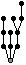
\includegraphics[scale=2]{desenhos/arvorerigidamae.png}
\end{center}

se associará ao conjunto $\{A,B,C\}$ onde $A,B,C$ são respectivamente os conjuntos de suas três filhas 

\begin{center}
        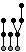
\includegraphics[scale=2]{desenhos/soasfilhas.png}
\end{center}

A filha do meio se associará ao conjunto que contém como único elemento o conjunto associado a sua única filha. Mas a sua filha é apenas um vértice, e portanto tem seu conjunto associado como sendo o $\varnothing$. Logo $B = \{\varnothing\}$. 

\begin{center}
        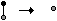
\includegraphics[scale=2]{desenhos/filhadomeio.png}
\end{center}


A filha da esquerda se associará ao conjunto que contém como único elemento o conjunto associado a sua única filha. A sua filha é a árvore com uma única aresta, que acabamos de descobrir no parágrafo anterior que se associa a $\{\varnothing\}$. Logo $A = \{\{\varnothing\}\}$.

\begin{center}
        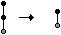
\includegraphics[scale=2]{desenhos/filhadaesquerda.png}
\end{center}

A filha da direita se associará ao conjunto que contém como elementos os conjuntos associados a suas duas filhas. Uma delas é a árvore com uma única aresta, e a outra é a árvore que é um único caminho de tamanho $2$, ambas as árvores que acabamos de encontrar seus conjuntos associados, $\{\varnothing\}$ e $\{\{\varnothing\}\}$. Logo $C = \{ \{\varnothing\}, \{\{\varnothing\}\} \}$

\begin{center}
        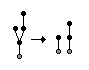
\includegraphics[scale=2]{desenhos/filhadadireita.png}
\end{center}


Uma simetria da árvore corresponderia a um conjunto com dois elementos formalmente iguais, mas que estariam sendo considerados como diferentes (como um multiconjunto, se conhece esta definição). Ao tentar encontrar um conjunto associado como no algoritmo que acabamos de descrever, a simetria iria se manifestar em algum momento onde ao encontrarmos as filhas de alguém, teriamos duas árvores iguais como filhas. Esse também é o motivo que a analogia das caixas mais cedo não capturava exatamente o que queríamos. Uma caixa com duas caixas vazias faz sentido, mas isto traduzido para conjuntos seria um conjunto com dois elementos, e ambos os elementos são o conjunto vazio. Em árvores, isso traduziria na raiz conectada a exatamente dois vértices - a bijeção que troca estes dois vizinhos é uma simetria, que em algum sentido captura a noção de igualdade entre as duas caixas vazias.

Certo, temos então o mesmo grafo, construído de duas formas diferentes. Esse grafo é realmente interessante, de muitos jeitos, por mais que possa não parecer agora. A primeira grande propriedade que vamos ver nele: ele contém todos os outros grafos contáveis dentro dele, de forma não trivial. O que quero dizer com não trivial é o seguinte. Se pegarmos contáveis vértices e ligarmos todos eles entre si, obtemos o famoso grafo completo $K_\omega$. É claro que todo grafo contável vai estar lá dentro desde que apaguemos vértices e arestas. O Grafo Contável tem a propriedade muito mais legal que conseguimos encontrar qualquer grafo contável lá dentro apagando apenas vértices, sem apagar arestas! Formalmente, o que estamos dizendo é que qualquer grafo contável é subgrafo induzido do Grafo Contável.


\begin{definicao*}[Subgrafo e subgrafo induzido]
    Um grafo $H$ é subgrafo de um grafo $G$ se seu conjunto de vértices e seu conjunto de arestas são subconjuntos dos de $G$. $H$ é subgrafo induzido se seu conjunto de vértices e subconjunto do de $G$ e todas as arestas existentes em $G$ entre estes vértices também são arestas de $H$.
\end{definicao*}

No linguajar dos logicistas, uma estrutura com uma certa propriedade (nesse caso, um grafo com a propriedade de ser contável), que contem como subestrutura todas as outras estruturas com a mesma propriedade (contém como subgrafo induzido todos os outros grafos contáveis) é conhecida como uma estrutura universal. No linguajar dos teoristas de categoria, uma propriedade que caracteriza unicamente um objeto a menos de isomorfismo é conhecida como uma propriedade universal. Sem medo de confusão entre tribos, vou usar os dois termos ao mesmo tempo: vamos agora encontrar uma propriedade universal pro Grafo Contável pra demonstrar sua universalidade.

\begin{proposicao}[Propriedade universal do Grafo Contável]
Existe um único grafo contável, a menos de isomorfismo, que satisfaz a seguinte propriedade: dados dois subconjuntos finitos disjuntos de vértices $A,B$, existe um vértice que é adjacente a todos os vértices em $A$ e não é adjacente a nenhum vértice de $B$.
\end{proposicao}
\begin{prova}
Seja $R$ o grafo que construímos mais cedo, cujos vértices são conjuntos hereditariamente finitos e arestas são dadas pela relação de pertencimento. Seja $A,B$ dois subconjuntos finitos de vértices de $R$, digamos $A = \{X_1, \dots, X_n\}$ e $B = \{Y_1, \dots, Y_m\}$. Note que o próprio conjunto $A$ é um conjunto hereditariamente finito (construído no dia seguinte ao  maior dia de nascimento dentre os $X_i$), portanto é um vértice de $R$. Como cada $X_i \in A$, o vértice $A$ é adjacente a todos os $X_i$. $B$ e $A$ são disjuntos, então os $Y_i \notin A$, mas poderíamos ter possivelmente $A \in Y_i$ para algum $i$. Para remediar este problema, escolha algum conjunto hereditariamente finito $Z$ que não pertence a $\underset{y \in Y_1\cup \dots \cup Y_n}{\bigcup }y$ e também $Z \neq Y_i$ para todo $i$ (ou seja, $Z$ é alguém que não é $Y_i$ e nem elemento de nenhum conjunto em $Y_i$) Agora modificamos nosso $A$ para $\tilde{A} \defeq \{X_1, \dots, X_n, Z\}$ e assim devemos ter $\tilde{A} \notin Y_i$ e $Y_i \notin A$ para todo $i$, garantindo finalmente que $\tilde{A}$ é nosso vértice procurado.

Para demonstrar a unicidade, usamos a famosa técnica do vai-e-vem. O truque é construir a função por passos, onde nos passos pares garantimos que ela vai cobrir todo o domínio que queremos e nos passos ímpares garantimos que ela vai cobrir toda a imagem que queremos. Tome dois grafos contáveis $R$ e $R'$ com a propriedade universal. Construiremos o isomorfismo por indução. Suponha que já temos um isomorfismo $f_i$ de um subgrafo induzido finito $X_i $ de $R$ em um subgrafo induzido finito $Y_i$ de $R'$ (para o primeiro passo, comece com uma função $f_1$ que manda um vértice qualquer de $R$ em outro vértice qualquer de $R'$). Se $i$ for ímpar, construa $f_{i+1}$ da seguinte maneira: tome algum vértice $v$ que não esteja em $X_i$. Seja $A$ os vértices de $X_i$ adjacentes a $v$ e $B$ os vértices de $X_i$ não adjacentes a $v$. Assim, suas imagens $f(A)$ e $f(B)$ em $Y_i$ são conjuntos finitos disjuntos e portanto pela propriedade universal de $R'$ existe um $v' \in R'$ que é adjacente a todos os $f(A)$ e nenhum dos $f(B)$. Defina $f_{i+1}(v) = v'$, $X_{i+1} = X_i \cup \{v\}$ e $Y_{i+1} = Y_i \cup \{v'\}$. No caso onde $i$ é par, fazemos a mesma coisa, porém agora começando a partir de um $v'$ em $R'$ que não está no $Y_i$ e usando a propriedade universal de $R$ para encontrar um $v$. Como ambos $R$ e $R'$ são contáveis, este processo garante que todos os vértices de $R$ e todos os vértices de $R'$ são cobertos quando tomamos a função $f$ como a união de todas as $f_i$, que assim será um isomorfismo.
\end{prova}

Percebeu que começamos a demonstração do isomorfismo entre $R$ e $R'$ mandando um vértice qualquer em outro vértice qualquer? Isso mostra que dados quaisquer par de vértices, conseguimos construir um automorfismo de $R$ que leva um no outro. Ou seja, todos os vértices são `iguais', no sentido de que existem simetrias que trocam quaisquer um deles entre si - esta é uma propriedade conhecida como transitividade. Na verdade, a demonstração consegue mostrar que $R$ possui um nível de simetria ainda mais alto que isso.

\begin{exercicio}
    \luafacil Sejam $X_1$ e $X_2$ dois subgrafos induzidos finitos de $R$ e $f:X_1 \rightarrow X_2$ um isomorfismo entre eles. Mostre que $f$ se estende para um automorfismo $f^*: R \rightarrow R$ (Dica: adapte a construção do isomorfismo da proposição anterior)
\end{exercicio}

Esta propriedade é conhecida como homogeneidade e é o maior nível de simetria que uma estrutura pode ter: quaisquer duas partes pequenas que se parecem podem ser levadas uma na outra por uma simetria da estrutura toda. Vamos falar de transitividade, homogeneidade e outras formas de grafos bem simétricos no próximo capítulo.

Voltando a universalidade de $R$.

\begin{proposicao}[Universalidade do Grafo Contável]
    Seja $X$ qualquer grafo contável. Então $X$ é isomorfo a um subgrafo induzido de $R$.
\end{proposicao}
\begin{prova}
Enumere os elementos de $X$ como $X = \{x_1, \dots, x_n, \dots\} $. Tome um vértice $v_1$ qualquer de $R$ e defina $f_1$ como a função que leva $x_1$ a $v_1$. Por indução, suponha que já temos um isomorfismo $f_i$ entre o subgrafo induzido $X_i$ em $X$ de $x_1, \dots, x_i$ e um subgrafo induzido $X'_i$ em $R$. Seja $A$ o conjunto de vértices de $X_i$ adjacentes a $x_{i+1}$ e $B$ o conjunto de vértices de $X_i$ não adjacentes a $x_{i+1}$. Então $f_i(A)$ e $f_i(B)$ são dois conjuntos finitos disjuntos de vértices de $R$ e portanto existe um $v_{i+1}$ adjacente a todos os $f_i(A)$ e não adjacente a todos os $f_i(B)$. Defina $X_{i+1}$ como o subgrafo induzido de $\{x_1, \dots, x_{i+1}\}$, e $X'_{i+1}$ com o subgrafo induzido de $X'_i \cup \{v_{i+1}\}$, e aí estenda $f_i$ para o isomorfismo $f_{i+1}$ entre $X_{i+1}$ e $X'_{i+1}$ mandando $x_{i+1}$ em $v_{i+1}$. Se $X$ for finito, eventualmente este processo termina em uma função $f$, caso contrário tome $f$ como a união de todas as funções $f_i$ - este $f$ é um isomorfismo de $X$ em um subgrafo induzido de $R$.
\end{prova}

Vamos finalizar esta história pincelando mais algumas construções surpreendentes do Grafo Contável. Continuando no tema de lógica, uma consequência interessante da construção do conjunto $V_\omega$ de conjuntos hereditariamente finitos é que ele consegue mostrar a independência de um dos axiomas de ZFC.

\begin{exercicio}
    \luamedio Mostre que $V_\omega$ é um modelo pra ZFC tirando o Axioma do Infinito (lembrando que assumimos na nossa metateoria que os axiomas de ZFC valem).
\end{exercicio}

Se analisarmos a demonstração da Propriedade Universal de $R$, dá para se ver que fato de $V_\omega$ satisfazer quase todos os axiomas de ZFC já é uma hipótese forte o suficiente para termos o resultado. Poderíamos, então, tomar como conjunto de vértices qualquer modelo contável de ZFC (sim, modelos contáveis do sistema inteiro, incluindo o Axioma do Infinito, `existem'!), e usar a sua relação de pertencimento como adjacência. Incrivelmente, isto resulta no Grafo Contável. Não é esquisito que exista um modelo contável de ZFC, sendo que dentro da teoria conseguimos mostrar a existência de conjuntos incontáveis? O próprio matemático que demonstrou o teorema que garante a existência de um modelo contável (teorema de Lowenheim-Skolem pra baixo) achou isso esquisito também (o `paradoxo de Skolem').

Outras áreas ainda mais distantes dão origem ao Grafo Contável. Tome como conjunto de vértices números primos que são congruentes a $1$ módulo $4$ (ou seja, ao dividir o primo por $4$ obtemos resto $1$). Ligamos $p$ com uma aresta a $q$ se $p$ é congruente modulo $q$ a algum número elevado ao quadrado $x^2$, ou o contrário, se $q$ é congruente modulo $p$ a algum número elevado ao quadrado (na verdade, a famosa `lei da reciprocidade quadrática' garante que estas condições são equivalentes, ou seja, a relação já era simétrica de começo). Usando alguns teoremas clássicos de teoria de números (teorema chinês dos restos, teorema de Dirichlet), é possível mostrar que este grafo satisfaz a Propriedade Universal.

Indo pra teoria de probabilidade: e se agora tomarmos como conjunto de vértices os números naturais, e construirmos um grafo aleatoriamente dando, pra cada par de vértices, probabilidade $1/2$ de existir uma aresta entre eles? Então, com probabilidade $1$ este processo resultará no Grafo Contável. Este resultado famoso motiva o nome mais comum na literatura para $R$, `o Grafo Aleatório'.

Não entramos em mais detalhes pra essas outras construções por que já viajamos longe demais da área da autora - nos contentamos com essa rápida pincelada e seguimos pro próximo tópico.

\section{Grafos de Simetrias}

\begin{center}
        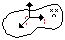
\includegraphics[scale=2]{desenhos/violencia.png}
\end{center}
Me foi transmitido, na minha época em meio aos geômetras, a fala do ancestral Hermann Weyl: ``A introdução de números como coordenadas é um ato de violência." A ideia aqui é que o espaço geométrico não possui coordenadas intrínsecas a si. Ele existe por si só, e podemos usar muitas diferentes formas de se colocar réguas (coordenadas) nele para facilitar nossa navegação. Pense, por exemplo, como diferentes regiões no mundo possuem diferentes sistemas de medida (metros, pés, polegadas, etc). A geometria moderna construiu uma linguagem sofisticada para se estudar espaços sem ter que violentamente introduzir coordenadas.

Vamos ir na direção contrária aqui. Vamos cometer o ato pecaminoso de introduzir algo análogo a coordenadas, mas agora não em um espaço, e sim em um grupo. 

A ideia de um sistema de coordenadas é fazer uma escolha arbitrária de direções, que serão consideradas como sendo de tamanho unitário. Assim, todas as outras direções de diferentes tamanhos possíveis são medidas com base na escolha inicial arbitrária de direções unitárias (em linguagem de Álgebra Linear: uma escolha de base para seu espaço vetorial). 

Para grupos, essa escolha de direções será uma escolha de elementos geradores. Se temos um subconjunto $S \subset G$ tais que todos os outros elementos podem ser escritos como produto de elementos de $S$, então dizemos que $S$ gera $G$ e seus elementos são os geradores. Assim, todo elemento de $G$ vira uma palavra com letras em $S$. Mas veja que esses elementos não precisam ser `independentes' - podem haver relações entre eles, e assim diferentes palavras podem representar o mesmo elemento de $G$.

Com estas coordenadas, agora podemos desenhar nosso grupo! Escolha uma cor pra cada elemento $s$ de $S$. Tome algum ponto qualquer no plano, e associe ele ao elemento identidade do grupo. Desenhe setas da cor de cada $s$ saindo da identidade e chegando em pontos nomeados como $s$. Agora, em um ponto nomeado com $s$, desenhe setas da cor de cada $s' \in S$ e faça estas setas chegarem em um ponto nomeado com o produto $s's$. Se já existir algum ponto com este nome, não crie um ponto novo, ligue a seta a ele. Faça isto até você criar pontos para todos os elementos do grupo. Este é o grafo de simetrias de $G$ em relação a $S$, mais normalmente conhecido como o grafo de Cayley de $G$ em relação a $S$.

Veja que falamos de setas ao invés de arestas, e que estamos colorindo nossas setas: estamos direcionando e colorindo nossos grafos.

\begin{definicao*}[Grafos Direcionados e Aresta-Coloridos]
    Um grafo direcionado $G$ consiste de um par de conjuntos $V,A$, onde $A$ é um subconjunto de $V\times V$. (agora sem precisar pedir que a relação é simétrica). Os elementos de $V$ são chamados vértices e os de $A$ de arestas direcionadas ou setas. Quando existe uma seta entre dois vértices $v$ e $w$, dizemos que eles são adjacentes e denotamos como $v \rightarrow w$.

\begin{center}
        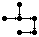
\includegraphics[scale=2]{desenhos/direcionado.png}
\end{center}

    Um grafo aresta-colorido é um grafo (direcionado ou não) com um conjunto de cores $C$ e uma função do conjunto de arestas (ou setas) para $C$.

\begin{center}
        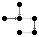
\includegraphics[scale=2]{desenhos/direcionadocolorido.png}
\end{center}
\end{definicao*}

\begin{definicao*}[Grafo de simetria, ou, grafo de Cayley]
Seja $G$ um grupo e $S\subset G$. O grafo de simetrias (ou de Cayley) direcionado e colorido de $G$ em relação a $S$ é o grafo cujo conjunto de vértices é $G$, o conjunto de cores é $S$, e existe  uma aresta direcionada de $g$ para $h$ colorida por $s$ se existir algum $s \in S$ tal que $g = hs$. Denotamos este grafo como $\overrightarrow{\text{Cay}}(G,S)$.

O grafo de simetrias, ou grafo de Cayley, de $G$ em relação a $S$ é o grafo cujo conjunto de vértices são os elementos de $G$, e existe uma aresta ligando $g$ a $h$ se existir algum $s \in S$ tal que $g = hs$. Denotamos este grafo como $\text{Cay}(G,S)$
    
\end{definicao*}

\begin{exercicio}
    \luafacil Se convença que esta definição é a mesma da construção descrita no parágrafo anterior, no caso onde $S$ gera $G$.
\end{exercicio}

Antes de irmos para os exemplos, uma parada para coletarmos um conceito relevante. Primeiro, concorda que se um $S$ gera $G$, então podemos ver os elementos de $G$ como palavras com letras em $S$? Pra deixar isso mais claro, vamos pegar um exemplo concreto. Tome $G$ o grupo de automorfismos do grafo que é um ciclo de quatro vértices.
    \begin{center}
        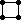
\includegraphics[scale=2]{desenhos/quadrado.png}
\end{center}

Nomeamos seus vértices para encontrarmos seu grupo de automorfismos

    \begin{center}
        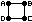
\includegraphics[scale=2]{desenhos/quadradonome.png}
\end{center}

Se brincar um pouco com isso, não vai demorar muito para se convencer que os automorfismos desse grafo coincidem exatamente com as isometrias do quadrado. Temos a identidade e as três rotações no sentido anti-horário de 90, 180 e 270 graus

\begin{align*}
    id:&            &  r_{90}:&              &  r_{180}:&     & r_{270}:& \\
A&\mapsto A           &  A&\mapsto B               &  A&\mapsto C & A &\mapsto D\\
B&\mapsto B         &  B&\mapsto C    &  B&\mapsto D & B &\mapsto A\\
C&\mapsto C  &  C&\mapsto D           &  C&\mapsto A & C &\mapsto B \\
D&\mapsto D  &  D&\mapsto A          &  D&\mapsto B  & D &\mapsto C
\end{align*}

E temos as quatro reflexões

\begin{align*}
    s_1:&            &  s_2:&              &  s_3:&     & s_4:& \\
A&\mapsto B           &  A&\mapsto C               &  A&\mapsto D & A &\mapsto A\\
B&\mapsto A         &  B&\mapsto B    &  B&\mapsto C & B &\mapsto D\\
C&\mapsto D  &  C&\mapsto A           &  C&\mapsto B & C &\mapsto C \\
D&\mapsto C  &  D&\mapsto D          &  D&\mapsto A  & D &\mapsto B
\end{align*}

sobre os eixos

    \begin{center}
        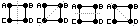
\includegraphics[scale=2.2]{desenhos/eixosquadrado.png}
\end{center}


Com um pouco de conta, dá para nos convencermos que basta a rotação de 90 graus $r \defeq r_{90}$ e qualquer uma das reflexões, digamos $s \defeq s_1$, para obtermos qualquer outro automorfismo.

\begin{align*}
id&=r^0           &  s_1 &= s             \\    
r_{90}&=r           &  s_2 &= rs             \\
r_{180}&=r^2         &  s_3&=r^2s   \\
r_{270}&=r^3    &  s_4&=r^3s          
\end{align*}
Ou seja, mostramos que $S = \{r,s\}$ é um subconjunto gerador de $G$. 

Agora, é claro que $r^4 = 1$. Talvez menos claro mas ainda facilmente verificável, $sr = r^3s$. Menos claro ainda: qualquer outra possível igualdade entre elementos de $G$ pode ser derivada apenas a partir destas duas. Por exemplo, podemos verificar que $sr^2= s_3$ olhando para as bijeções. E portanto $sr^2 = s_3 = r^2s$. Mas essa mesma igualdade segue das manipulações

\[
sr^2 = srr = r^3sr = r^3r^3s = r^6s = r^2s
\]

onde usamos apenas as duas igualdades $sr = r^3s$ e $r^4 = 1$.

Como poderíamos mostrar que qualquer igualdade é derivável apenas destas duas igualdades? Podemos fazer o seguinte: construimos um grupo onde esse fato é válido. E aí mostramos que esse grupo é isomorfo a nosso $G$.

Por simplicidade de exposição (mais vulgarmente conhecido como preguiça da autora, ou apelando pra limitações de recursos naturais, falta de papel e tinta), vou dar apenas a intuição de como isso é feito, sem formalizar. Este é o tipo de coisa que é perfeitamente claro intuitivamente, e perfeitamente confuso formalmente.

Se temos um conjunto $A$ qualquer, podemos construir $F(A)$, o dito grupo livre sobre $A$. Imaginamos $A$ como um alfabeto, e seus elementos como letras. Estendemos esse alfabeto, adicionando para cada letra $a \in A$ um símbolo formal $a^{-1}$ que simbolizará sua inversa. Os elementos de $F(A)$ serão palavras (strings) sobre esse alfabeto estendido. A operação de grupo aqui é concatenação de palavras - coloque uma na frente da outra. Por exemplo, se $A = \{a,b\}$, então $abba^{-1}b$ é uma palavra, $ab^{-1}$ é outra. A operação destas duas é $abba^{-1}bab^{-1}$. Com essa operação, a palavra `vazia' (sem letras) se torna a identidade, que denotamos como $1$. E o que acontece se concatenarmos $ab^{-1}$ com $ba$? Na verdade, mentimos na definição desse parágrafo. Precisamos quocientar as palavras pelo processo de redução: $ab^{-1}ba$ deveria ser igual a $aa$, tornando assim a inversa antes puramente formal em uma inversa de verdade (se concatenarmos $a$ com $a^{-1}$ a redução a torna a palavra vazia).  Chamamos esta criatura de grupo livre porque ele é `livre' de quaisquer equações não triviais - as triviais sendo exatamente as dadas pela redução de palavras.

Talvez vai existir um apêndice com a construção formal (e categórica) do grupo livre. Talvez não.

De posse do grupo livre, conseguimos criar grupos muito facilmente, simplesmente demandando equações novas pro $F(A)$ (formalmente, se temos uma equação $x = y$ entre palavras $x,y$, quocientamos $F(A)$ pelo subgrupo normal gerado por $xy^{-1}$). Voltando ao exemplo do quadrado, e se tomarmos $A$ como sendo as letras $r,s$ e criassemos o grupo $\tilde{G}$ como sendo o quociente de $F(A)$ pelas equações $r^4 = 1$ e $sr = r^3s$? Geralmente, essa é a notação usada para esse tipo de construção $\tilde{G} \defeq \langle r,s \mid r^4 = 1, sr = r^3s \rangle$

\begin{exercicio}
\luamedio Se convença que $G \cong \tilde{G}$
\end{exercicio}

Encontrar elementos geradores e equações completas (que implicam em qualquer outra equação) é super útil, e é geralmente chamado de encontrar uma apresentação para o grupo.


\begin{definicao*}[Geradores, apresentação de um grupo e grupo livre]
    Dado um grupo $G$ e um subconjunto $S \subset G$, dizemos que $S$ gera $G$ se todo elemento de $G$ é um produto de elementos de $S$.

    Uma apresentação de $G$ é um par $S$ e $R$ onde $S$ é um subconjunto gerador de $G$ e $R$ é um conjunto de igualdades entre produtos de elementos de $S$, de forma que qualquer possível igualdade em $G$ pode ser derivada a partir de igualdades em $R$. Se $S = \{s_1, \dots, s_n\}$ e $R = \{r_1, \dots, r_m \}$ então escrevemos $G = \langle s_1, \dots, s_n \mid r_1, \dots, r_m \rangle$.

    Se $G$ admite uma apresentação onde $R$ é vazio, dizemos que $G$ é um grupo livre, e dizemos que seu conjunto gerador $S$ gera $G$ livremente. 


\end{definicao*}


\begin{exemplo*}
\begin{itemize}[label=\ding{212}]
    \item O grupo que estavamos falando mais cedo, dos automorfismos do ciclo de quatro vértices, ou equivalentemente as isometrias do quadrado, é conhecido como $D_4$. Usando sua apresentação $D_4 = \langle r,s \mid r^4 = 1, sr = r^3s \rangle$, podemos facilmente desenhar seu grafo $\overrightarrow{\text{Cay}}(G,S)$ tomando $S = \{r,s\}$. O vértice destacado é o referente a identidade, a cor mais escura das arestas é a referente ao $r$ e a cor mais clara referente ao $s$.
    
    \begin{center}
        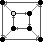
\includegraphics[scale=2]{desenhos/d4colorido.png}
\end{center}

    E seu grafo sem cores e direções $\Cay(G,S)$

     \begin{center}
        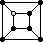
\includegraphics[scale=2]{desenhos/d4semdirecaocor.png}
\end{center}

    Coincidentemente (será?) é o grafo da projeção do cubo.
    \item Os números inteiros $\mathbb{Z}$ formam um grupo usando a operação de adição. Como qualquer número inteiro $n$ é a soma de vários $1$ ou vários $-1$, então $S = \{1,-1\}$ é gerador de $\mathbb{Z}$. Assim, $\mathbb{Z}$ admite uma apresentação muito trivial:  $\mathbb{Z} = \langle a \rangle = F(\{a\})$, ou seja, é o próprio $F(A)$ sem equações a mais, no caso onde $A$ possui uma única letra. Denotando a identidade (que é apenas o número $0$) como o vértice destacado novamente, seu grafo colorido e direcionado é
\begin{center}
    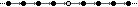
\includegraphics[scale=1.7]{desenhos/zcolorido.png}
\end{center}
e quando apagamos as cores e direções obtemos o raio duplo.
     \begin{center}
        
\includegraphics[scale=1.7]{desenhos/zsemcordirec.png}
\end{center} 
    \item E se tomarmos agora o $F(A)$ novamente mas agora com $A$ tendo dois elementos, digamos $A = \{a,b\}$? Obtemos uma árvore, onde todos os vértices possuem exatamente $4$ vizinhos (`a árvore $4$-regular')
    
 \begin{center}
        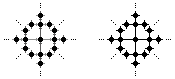
\includegraphics[scale=2]{desenhos/2freegroup.png}
\end{center} 

    Aqui se esconde toda um mundo de conexões com geometria hiperbólica. Falando sobre isso...
    \item ... um dos grupos mais famosos da matemática, que parece estar conectado com todas as suas áreas, é o Grupo Modular $\Gamma$. Ele pode ser apresentado como $\Gamma = \langle a,b \mid a^3 = 1, b^4 = 1 \rangle$. Seu grafo sem cores e direções, pra facilitar o (difícil) desenho:
    
     \begin{center}
        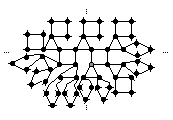
\includegraphics[scale=2]{desenhos/modular.png}
\end{center} 

    Vê o padrão? Todo vértice está (ou deveria estar, se eu tivesse papel e lápis infinitos) em exatamente um triângulo e um quadrado. Colando infinitamente triângulos e quadrados dessa forma, obtemos o grafo.
\end{itemize}
    
\end{exemplo*}

Grupos infinitos, porém gerados por finitos elementos, aparecem naturalmente em muitos lugares da matemática, principalmente na topologia algébrica e na geometria. Seus grafos associados são, então, um dos lugares mais comuns para que um matemático usual possa tropeçar em um grafo infinito. Ao transformar um objeto algébrico em um objeto combinatório (ou geométrico - uma técnica de estudo é metrizar o grafo postulando que todas as arestas tem tamanho $1$), conseguimos traduzir problemas algébrico em outra linguagem e assim obter insights novos. Um exemplo simples dessa tradução:

\begin{exercicio}
    \luafacil Mostre que o grafo de simetria de $G$ em relação a $S$ é conexo se e somente se $S$ é gerador de $G$.
\end{exercicio}


Um outro exemplo simples desse fenômeno você já possa ter percebido ao analisar os exemplos dados: as relações de uma apresentação de um grupo se transformam em ciclos no grafo. No grafo de $D_4$, a relação $r^4 = 1$ se torna um ciclo de quatro vértices (a `face frontal' do cubo)

     \begin{center}
        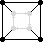
\includegraphics[scale=2]{desenhos/d4facefrontal.png}
\end{center} 

e a relação $sr = r^3s$ também se torna um ciclo de quatro vértices (a `face lateral' do cubo).

     \begin{center}
        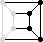
\includegraphics[scale=2]{desenhos/d4facelateral.png}
\end{center} 

Nos dois grupos livres $\mathbb{Z}$ e $F(\{a,b\})$, como não temos relações, não temos ciclos. E no grupo modular $\Gamma = \langle a,b \mid a^3 = 1, b^4 = 1 \rangle$, a relação $a^3 = 1$ dá origem aos triângulos (ciclos de três vértices) e $b^4 = 1$ dá origem aos quadrados (ciclos de quatro vértices)

Vamos nos próximos capítulos estudar versões mais sofisticadas desse jogo de traduções entre grupos e grafos.


\end{document}
